\renewcommand{\thechapter}{\arabic{chapter}}
\setcounter{chapter}{7}

\chapter{Approche multimodale}
\label{chap:chapter_8}
\chapterintro
Les travaux de la précédente partie ont porté sur le diagnostic de données malignes sur la modalité de \acrlong{rcm}, plus particulièrement de pathologies de \acrlong{lm} et de \acrlong{lmm}. Au premier niveau hiérarchique, soit celui des images, ces chapitres ont permis la mise en avant de méthodes de séparation des tissus sains, bénins et malins. Au second niveau hiérarchique, soit celui des lésions, ces méthodes permettent la prédiction des pathologies bénignes et malignes.\par

Ce nouveau chapitre rempli l'objectif de ce manuscrit en intégrant une dimension multimodale au processus de prise de décision. Tout d'abord, les aspects d'extraction de caractéristiques et de diagnostic par le biais de modèles de prédiction est traité pour chacune des modalités présentes dans le jeu de données utilisé. De plus, la calibration de ces modèles de prédiction est envisagée afin de rendre cohérent les décisions entre chacun d’entre eux. Puis, les systèmes multimodaux envisagés dans ce travail sont présentés selon deux axes~: une première méthode qualifiée comme sans mémoire, puis une seconde méthode qualifiée sous le terme d’avec mémoire. Finalement, les résultats obtenus à l'aide de ces méthodes sont présentés et discutés.\par
\newpage

\section{Méthodologie}
Lors de la \Cref{part:microscopy}, diverses méthodes de classification ont été proposées afin de gérer les données issues de la modalité \gls{rcm} soit au niveau des images, soit au niveau des lésions. Outre le besoin de lever un certains nombre de verrous scientifiques, la réalisation de ces travaux a constitué une étape nécessaire à la réalisation du processus multimodal de ce manuscrit. Néanmoins à ce stade des travaux, les diverses méthodes proposées par ce manuscrit et par la littérature ne permettent que la prédiction au niveau d'une modalité et indépendemment de chacune d'entre elles.\par

Ce dernier chapitre propose une méthodologie en plusieurs temps pour permettre la mise en place d'un processus d'aide au diagnostic multimodal.

Pour parvenir à la réalisation de ce processus de décision multimodal, ce manuscrit propose de détailler les divers étapes qui le compose. Dans un premier temps, ce chapitre propose une mise au point sur les techniques permettant un diagnostic sur les modalités employé dans ce manuscrit. Dans un second temps, le principe de la calibration de modèle est présenté, dont l'utilisation est recommandé dans des contextes impliquant la collaboration de multiples modèles de prédiction. Dans un troisième temps, les processus multimodaux de prise de décision élaborés pour le besoin de cette problématique sont présentés, avec d'une part la considération d'un processus sans mémoire et d'autre d'un processus avec mémoire. Pour finir, ce chapitre se termine par une présentation des résultats issues des méthodes proposées, suivi d'une discussion sur ceux-ci.\par 

\section{Diagnostic des modalités}
\subsection{Diagnostic sur photographie clinique et de dermatoscopie}
\subsection{Diagnostic sur microscopie confocale}
\clearpage

\section{Calibration de modèles}
La majeure partie des modèles de classification mettent à disposition des scores représentant l'appartenance à chacune des classes de la problématique visée. Ces scores sont à l'origine des prédictions de ces modèles et peuvent être obtenus de manière complémentaire à la prédiction. Ainsi, la classe n'est bien souvent que la manifestation de la classe ayant achevé le score le plus élevé.\par

Malheureusement, ces scores n'ont de sens que dans le contexte dans lequel ils ont été obtenus et ne conviennent pas lorsque plusieurs sources d'information différentes sont combinées. Ainsi, une estimation précise de la \textbf{probabilité} d'appartenance à chacune des classes est un indicateur plus pertinent dans ce type de stituation, ayant un sens en dehors du champ d'action propre à chacun de ces modèles~\cite{Zadrozny2002}.\par

Diverses méthodes sont proposées afin de transformer ces scores en probabilités, tout d'abord sur des problématiques binaires, puis plus tardivement sur des problématiques à classes multiples. Ce principe de transformation des scores en probabilités porte le nom de processus de \textbf{calibration}.\par

Ainsi, les méthodes de la littérature sont multiples
Isotonic regression, \cite{Zadrozny2002}
Bayesian Binning into Quantiles (BBQ) calibration\cite{Naeini2015}
Beta calibration,\cite{Kull2017}
Sigmoid,\cite{kull2017b}

\section{Système multimodal}
\subsection{Système séquentiel sans mémoire}
\subsection{Système séquentiel avec mémoire}

\section{Présentation des résultats}
Cette section se destine à la présentation des résultats issus des méthodes précédemment énoncées. Dans un premier temps, 

Les précédentes sections de ce travail se sont consacrées à décrire des méthodes pour tenter de résoudre la problématique de prédiction au niveau des lésions à partir de données \gls{rcm}. Cette nouvelle section se dédie à la présentation des résultats pour donner suite aux diverses expérimentations mentionnées précédemment. Dans une première sous-section, le protocole d'expérimentation suivi pour permettre l'obtention des résultats est relaté et l'organisation de ces résultats est décrite. Puis dans une seconde sous-section, les divers résultats issus des expériences mentionnées précédemment sont développées.\par

\subsection{Protocole d’expérimentation}
Afin de réaliser l'évaluation de ces expériences, une \textbf{validation croisée imbriquée} est employée, déjà discutée lors de la \Cref{sec:models_settings}, pour ses avantages permettant ainsi l'obtention de métriques plus objectives sur les performances du système évalué~\cite{Cawley2010}. Ce type de structure de validation est plus robuste face au biais~\cite{Cawley2010} et est démontré empiriquement moins sensible au biais et à la variance lorsque celle-ci est couplée à des valeurs de $k$ comprises entre 5 et 10 pour l'évaluation~\cite{James2000}. La diversité de combinaisons relativement limitée de cette partie, permet à l'instar des précédents chapitres, d'obtenir des résultats dans un temps raisonnable malgré des valeur de $k$ élevées. Ainsi \textbf{une valeur de $k$ égale à 10} est utilisée pour l'évaluation, tandis qu'une valeur de 2 est conservée pour la boucle interne suffisante pour déterminer la meilleure combinaison d'hyperparamètres. Bien que considéré comme une possibilité, le schéma de validation de type \textit{leave-one-out} pour la boucle externe d'évaluation n'est pas utilisé car plus sujet à une variance élevée lors des mesures notamment en présence de valeurs aberrantes~\cite{Bengio2004}. De plus, un tel schéma de validation est bien plus coûteux à entreprendre puisqu'il nécessite autant de phases d'entraînement et d'évaluation, que d'instances dans le jeu de données considérée, soit 223 pour ce travail.\par

D'une part, pour procéder au mieux au réglage des paramètres des modèles précédents et, d'autre part, pour retenir une évaluation objective de ces processus malgré les déséquilibres d'annotations, il est nécessaire d'opter pour une métrique adaptée. Ces expériences emploient le \textbf{\fscore{}} permettant de représenter conjointement les mesures de précision et de rappel au sein d'une même métrique binaire. De plus, et afin de compléter l'analyse des résultats et de permettre un parallèle avec ceux des experts en dermatologie, les valeurs de \textbf{sensibilité} et de \textbf{spécificité} sont renseignées conjointement au \fscore{}. Comme pour l'article de Cinotti et al.~\cite{Cinotti2016}, ce processus décompose la présentation des résultats en deux temps. Dans un premier temps, est présentée l'analyse des mesures précédentes \textbf{sur l'ensemble des cas clinique} du jeu de données, en adoptant comme classe positive les annotations des lésions dites \textit{malignes}. Puis dans un second temps, les même mesures sont extraites \textbf{en ne considérant que les cas de \textbf{\gls{lm} / \gls{lmm}} parmi les annotations malignes} et en adoptant comme classe positive les annotations des lésions dites \textit{malignes}.\par

La partie dédiée aux résultats se décompose en diverses étapes, débutant dans un premier temps par une présentation des résultats obtenus \textbf{au niveau lésionnel par les diverses méthodes supervisées} présentée lors de la \Cref{sec:patient_decision_supervised}. Dans un second temps, ce travail procède à une présentation des résultats obtenus \textbf{au niveau lésionnel par l'utilisation des méthodes faiblement supervisées} listées lors de la \Cref{sec:patient_decision_weak}. En continuité de ces résultats sur les méthodes faiblement supervisées, ce travail procède à une analyse inversée par la méthode \gls{misvm}. Ainsi, ce travail évalue la qualité des prédictions au niveau des instances images, afin de déterminer la compréhension du phénomène à bas niveau par cette méthode.\par
\clearpage

\subsection{Résultats des expérimentation}

% Sequential - Pondéré
\begin{table}[H]
    \begin{tabular}{llllll}
        \toprule 
        Type                    & Modalité                          & Seuil             & Sans                  & Isotonic              & Sigmoid               \\ \midrule
        \multirow{4}{*}{Simple} & \multirow{2}{*}{Croissant}        & Croissant         & 0,72$\pm$0,14         & 0,65$\pm$0,14         & 0,66$\pm$0,10         \\ \cline{3-6}
                                &                                   & Décroissant       & 0,72$\pm$0,14         & 0,64$\pm$0,12         & 0,65$\pm$0,09         \\ \cline{2-6}
                                & \multirow{2}{*}{Décroissant}      & Croissant         & \textbf{0,81$\pm$0,08}& 0,61$\pm$0,11         & 0,79$\pm$0,10         \\ \cline{3-6}
                                &                                   & Décroissant       & 0,81$\pm$0,11         & 0,60$\pm$0,13         & 0,79$\pm$0,10         \\ \cline{1-6}
        \multirow{4}{*}{Double} & \multirow{2}{*}{Croissant}        & Croissant         & 0,71$\pm$0,09         & 0,64$\pm$0,18         & 0,71$\pm$0,13         \\ \cline{3-6}
                                &                                   & Décroissant       & 0,71$\pm$0,09         & 0,63$\pm$0,17         & 0,70$\pm$0,14         \\ \cline{2-6}
                                & \multirow{2}{*}{Décroissant}      & Croissant         & 0,77$\pm$0,13         & 0,71$\pm$0,16         & 0,77$\pm$0,12         \\ \cline{3-6}
                                &                                   & Décroissant       & 0,77$\pm$0,13         & 0,68$\pm$0,14         & 0,77$\pm$0,12         \\ \bottomrule
    \end{tabular}
\end{table}

% Sequential - Malignant
\begin{table}[H]
    \begin{tabular}{llllll}
        \toprule 
        Type                    & Modalité                          & Seuil             & Sans                  & Isotonic              & Sigmoid               \\ \midrule
        \multirow{4}{*}{Simple} & \multirow{2}{*}{Croissant}        & Croissant         & 0,79$\pm$0,10         & 0,76$\pm$0,09         & 0,79$\pm$0,07         \\ \cline{3-6}
                                &                                   & Décroissant       & 0,79$\pm$0,10         & 0,76$\pm$0,09         & 0,79$\pm$0,07         \\ \cline{2-6}
                                & \multirow{2}{*}{Décroissant}      & Croissant         & 0,85$\pm$0,11         & 0,74$\pm$0,07         & 0,85$\pm$0,10         \\ \cline{3-6}
                                &                                   & Décroissant       & 0,85$\pm$0,10         & 0,75$\pm$0,08         & \textbf{0,85$\pm$0,08}\\ \cline{1-6}
        \multirow{4}{*}{Double} & \multirow{2}{*}{Croissant}        & Croissant         & 0,80$\pm$0,07         & 0,77$\pm$0,11         & 0,78$\pm$0,10         \\ \cline{3-6}
                                &                                   & Décroissant       & 0,80$\pm$0,07         & 0,76$\pm$0,11         & 0,79$\pm$0,09         \\ \cline{2-6}
                                & \multirow{2}{*}{Décroissant}      & Croissant         & 0,83$\pm$0,11         & 0,80$\pm$0,11         & 0,83$\pm$0,09         \\ \cline{3-6}
                                &                                   & Décroissant       & 0,83$\pm$0,10         & 0,79$\pm$0,11         & 0,84$\pm$0,09         \\ \bottomrule    
    \end{tabular}
\end{table}


% Cumulative - Pondéré
\begin{table}[H]
    \begin{tabular}{llllll}
        \toprule 
        Type                    & Modalité                          & Seuil             & Sans                  & Isotonic              & Sigmoid               \\ \midrule
        \multirow{4}{*}{Simple} & \multirow{2}{*}{Croissant}        & Croissant         & 0,74$\pm$0,08         & 0,72$\pm$0,13         & 0,72$\pm$0,12         \\ \cline{3-6}
                                &                                   & Décroissant       & 0,72$\pm$0,09         & 0,74$\pm$0,14         & 0,70$\pm$0,13         \\ \cline{2-6}
                                & \multirow{2}{*}{Décroissant}      & Croissant         & 0,83$\pm$0,10         & 0,82$\pm$0,08         & 0,82$\pm$0,09         \\ \cline{3-6}
                                &                                   & Décroissant       & 0,82$\pm$0,10         & 0,81$\pm$0,08         & 0,80$\pm$0,12         \\ \cline{1-6}
        \multirow{4}{*}{Double} & \multirow{2}{*}{Croissant}        & Croissant         & 0,69$\pm$0,11         & 0,73$\pm$0,14         & 0,68$\pm$0,11         \\ \cline{3-6}
                                &                                   & Décroissant       & 0,68$\pm$0,12         & 0,72$\pm$0,12         & 0,68$\pm$0,13         \\ \cline{2-6}
                                & \multirow{2}{*}{Décroissant}      & Croissant         & \textbf{0,83$\pm$0,08}& 0,82$\pm$0,08         & 0,78$\pm$0,11         \\ \cline{3-6}
                                &                                   & Décroissant       & 0,82$\pm$0,08         & 0,81$\pm$0,08         & 0,78$\pm$0,12         \\ \bottomrule
    \end{tabular}
\end{table}

% Cumulative - Malignant
\begin{table}[H]
    \begin{tabular}{llllll}
        \toprule 
        Type                    & Modalité                          & Seuil             & Sans                  & Isotonic              & Sigmoid               \\ \midrule
        \multirow{4}{*}{Simple} & \multirow{2}{*}{Croissant}        & Croissant         & 0,82$\pm$0,06         & 0,81$\pm$0,09         & 0,81$\pm$0,09         \\ \cline{3-6}
                                &                                   & Décroissant       & 0,80$\pm$0,06         & 0,82$\pm$0,09         & 0,80$\pm$0,09         \\ \cline{2-6}
                                & \multirow{2}{*}{Décroissant}      & Croissant         & \textbf{0,87$\pm$0,06}& 0,86$\pm$0,06         & 0,85$\pm$0,08         \\ \cline{3-6}
                                &                                   & Décroissant       & 0,86$\pm$0,07         & 0,85$\pm$0,06         & 0,84$\pm$0,08         \\ \cline{1-6}
        \multirow{4}{*}{Double} & \multirow{2}{*}{Croissant}        & Croissant         & 0,79$\pm$0,08         & 0,81$\pm$0,10         & 0,78$\pm$0,08         \\ \cline{3-6}
                                &                                   & Décroissant       & 0,79$\pm$0,08         & 0,81$\pm$0,08         & 0,78$\pm$0,09         \\ \cline{2-6}
                                & \multirow{2}{*}{Décroissant}      & Croissant         & 0,86$\pm$0,06         & 0,86$\pm$0,06         & 0,83$\pm$0,09         \\ \cline{3-6}
                                &                                   & Décroissant       & 0,86$\pm$0,07         & 0,86$\pm$0,06         & 0,82$\pm$0,09         \\ \bottomrule
    \end{tabular}
\end{table}

\begin{figure}[H]
    \centering
    \includegraphics[width=\linewidth]{contents/chapter_8/resources/results_calibration_sequential.pdf}
    \caption{}
    \label{fig:results_calibration_sequential}
\end{figure}\par

\begin{figure}[H]
    \centering
    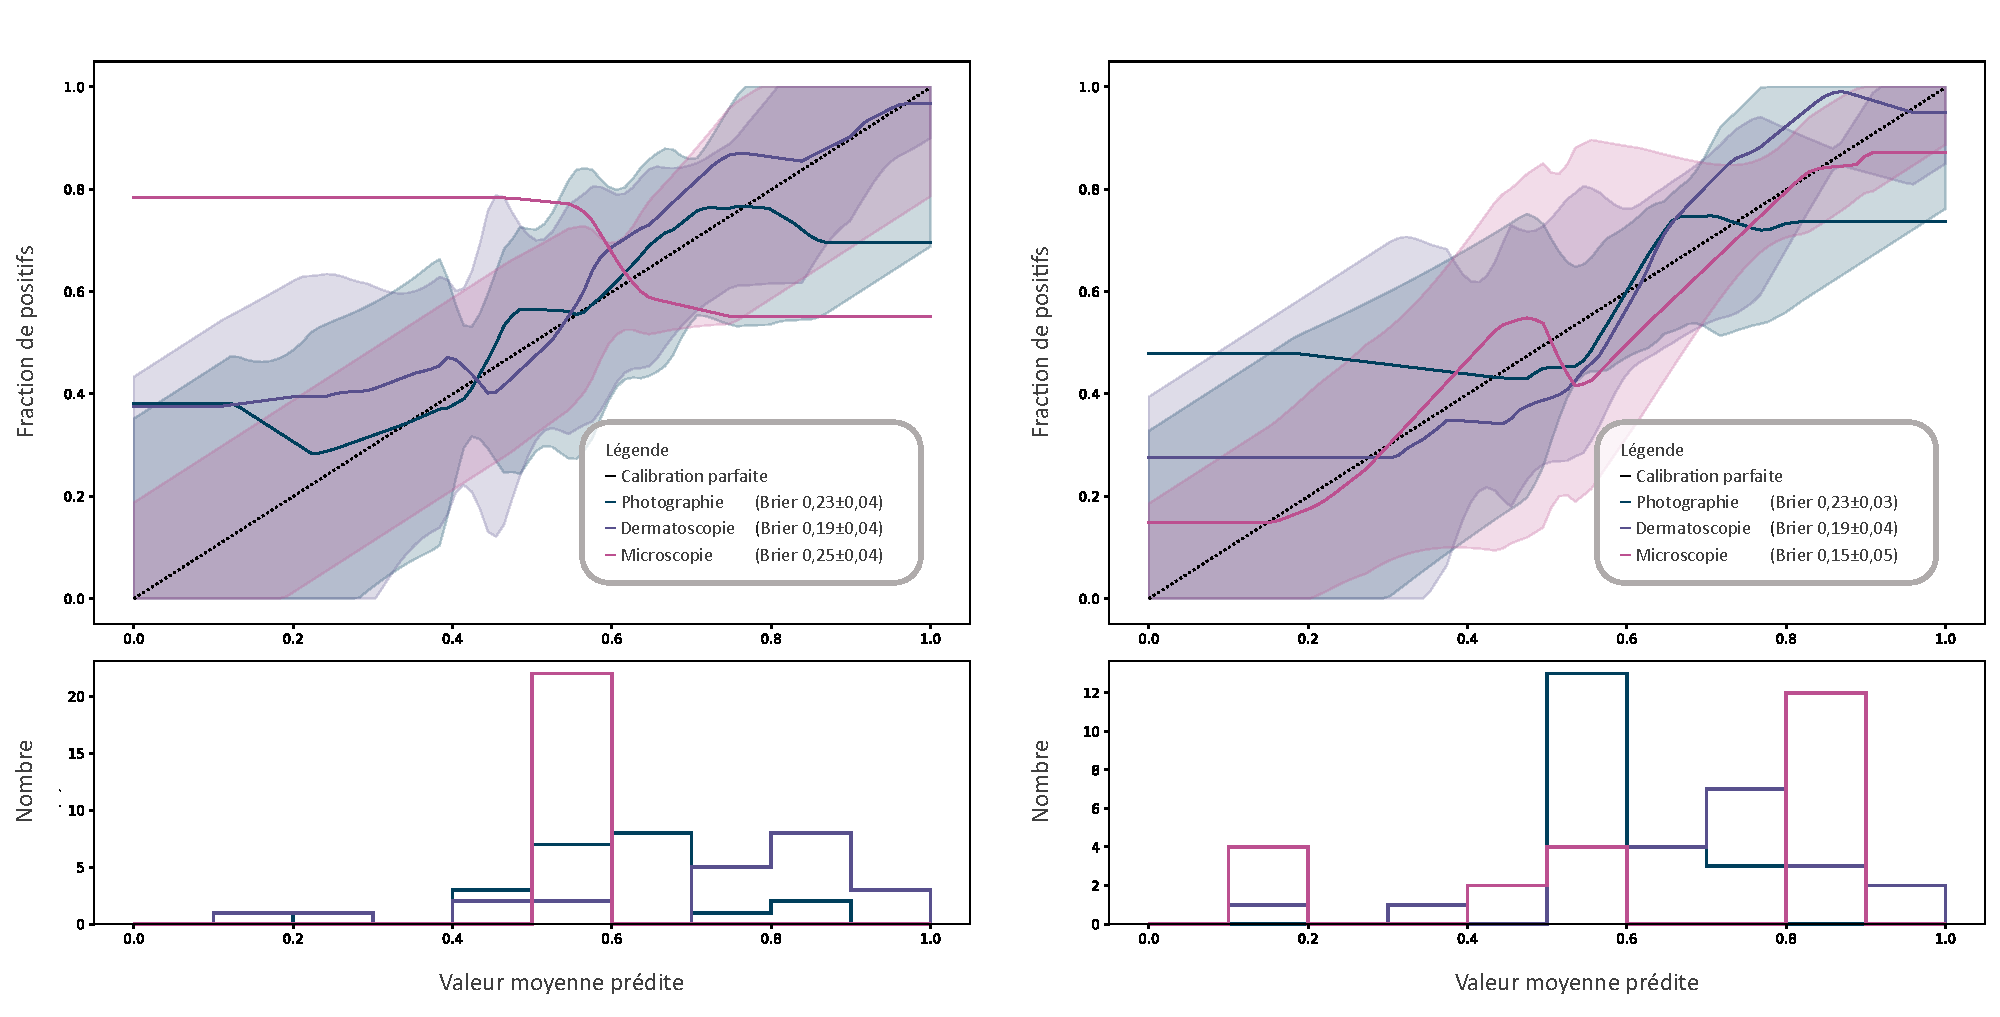
\includegraphics[width=\linewidth]{contents/chapter_8/resources/results_calibration_sequential_calibrated.pdf}
    \caption{}
    \label{fig:results_calibration_sequential_calibrated}
\end{figure}\par

\begin{figure}[H]
    \centering
    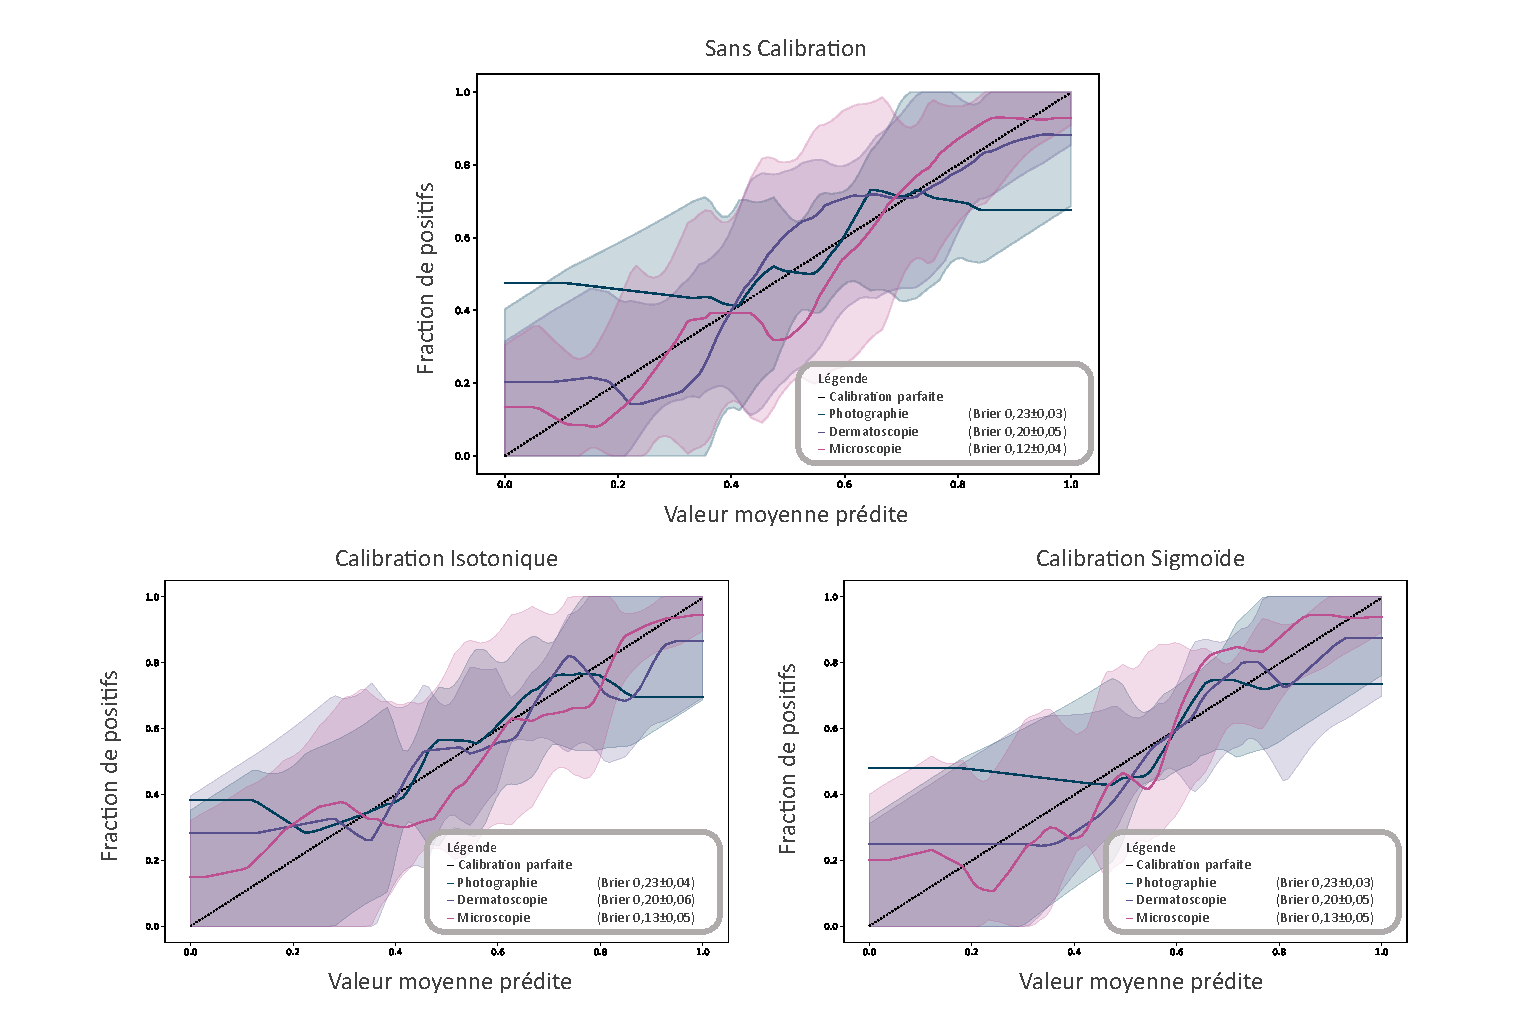
\includegraphics[width=\linewidth]{contents/chapter_8/resources/results_calibration_cumulative.pdf}
    \caption{}
    \label{fig:results_calibration_cumulative}
\end{figure}\par

\begin{figure}[H]
    \centering
    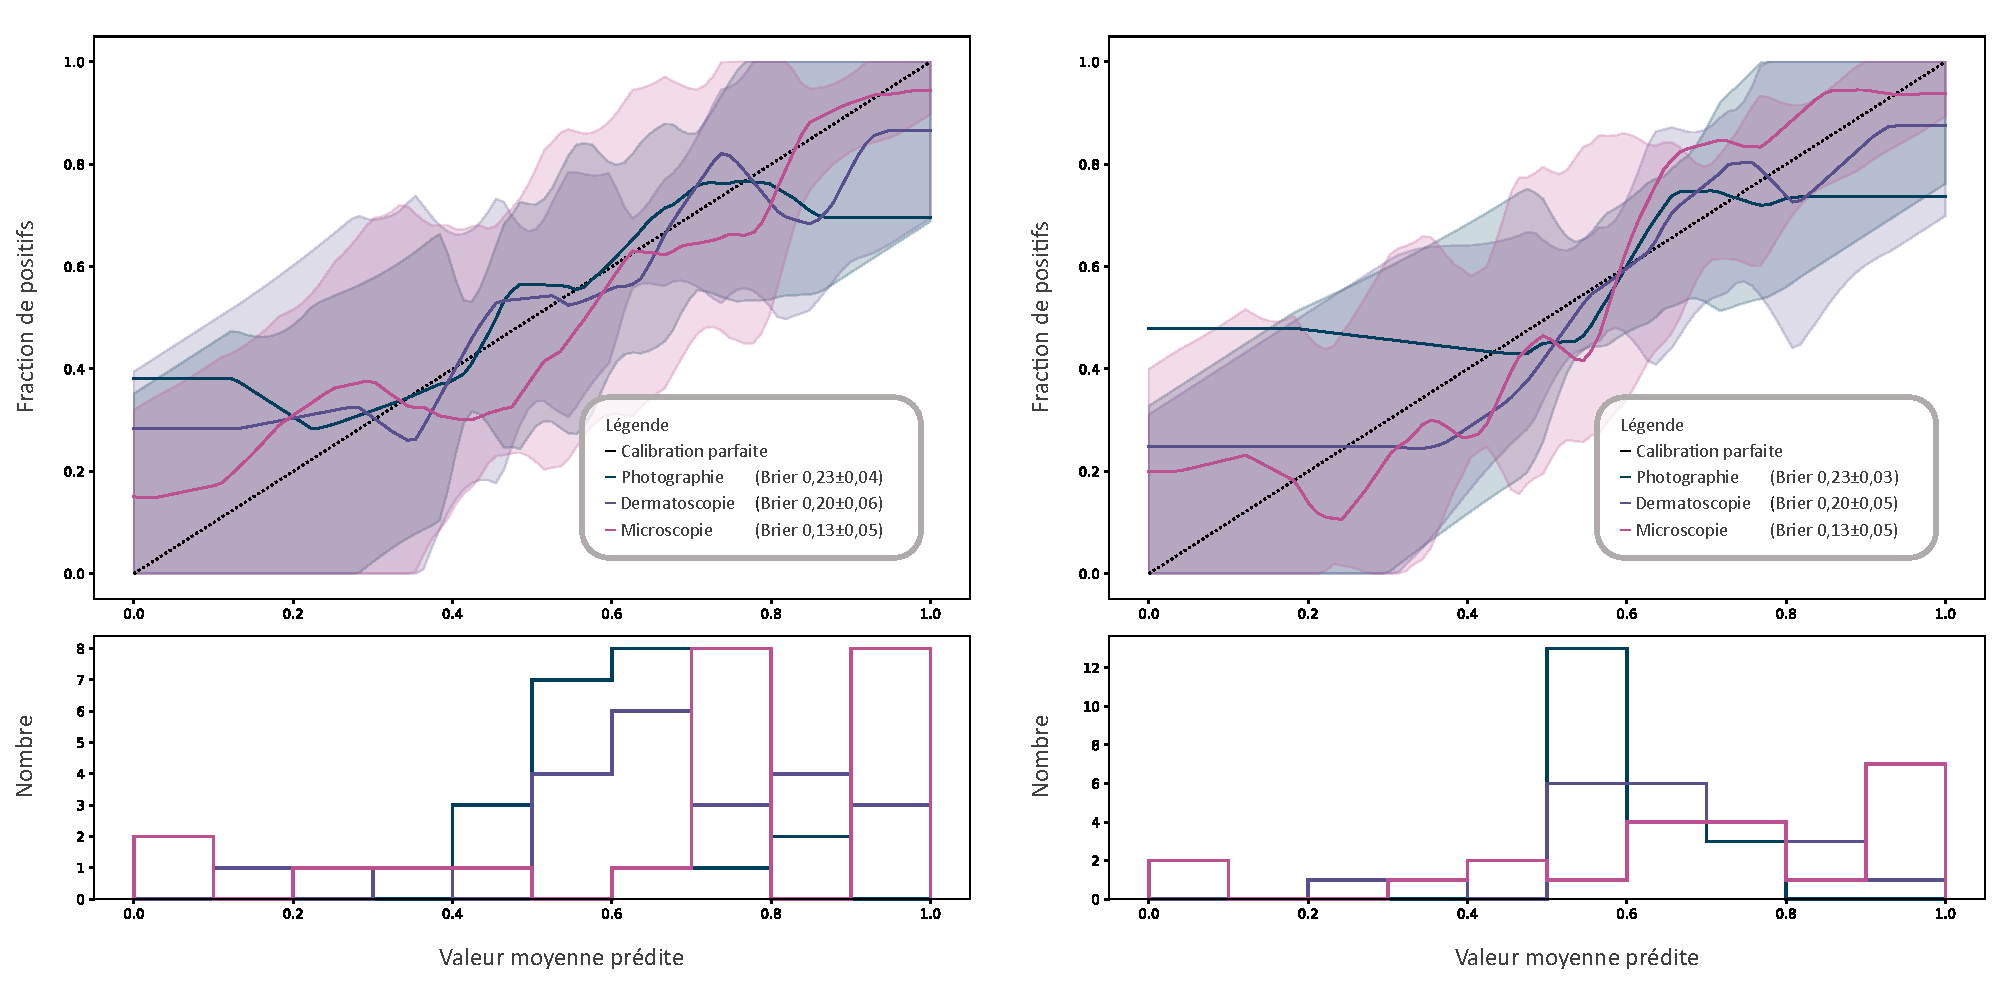
\includegraphics[width=\linewidth]{contents/chapter_8/resources/results_calibration_cumulative_calibrated.pdf}
    \caption{}
    \label{fig:results_calibration_cumulative_calibrated}
\end{figure}\par

\begin{figure}[H]
    \centering
    \includegraphics[width=\linewidth]{contents/chapter_8/resources/results_processus_weighted.pdf}
    \caption{}
    \label{fig:results_processus_weighted}
\end{figure}\par

\begin{figure}[H]
    \centering
    \includegraphics[width=\linewidth]{contents/chapter_8/resources/results_processus_malignant.pdf}
    \caption{}
    \label{fig:results_processus_malignant}
\end{figure}\par

\section{Discussion}